\documentclass[a4paper,11pt]{memoir}
%%%%%%%%%%%%%%%%%%%%%%%%%%%%%%%%%%%%%%%%%
% Wenneker Resume/CV
% Structure Specification File
% Version 1.1 (19/6/2016)
%
% This file has been downloaded from:
% http://www.LaTeXTemplates.com
%
% Original author:
% Frits Wenneker (http://www.howtotex.com) with extensive modifications by 
% Vel (vel@latextemplates.com)
%
% License:
% CC BY-NC-SA 3.0 (http://creativecommons.org/licenses/by-nc-sa/3.0/)
%
%%%%%%%%%%%%%%%%%%%%%%%%%%%%%%%%%%%%%%%%%

%----------------------------------------------------------------------------------------
%	PACKAGES AND OTHER DOCUMENT CONFIGURATIONS
%----------------------------------------------------------------------------------------

\usepackage{XCharter} % Use the Bitstream Charter font
\usepackage[utf8]{inputenc} % Required for inputting international characters
\usepackage[T1]{fontenc} % Output font encoding for international characters

\usepackage[top=1cm,left=1cm,right=1cm,bottom=1cm]{geometry} % Modify margins

\usepackage{graphicx} % Required for figures

\usepackage{flowfram} % Required for the multi-column layout

\usepackage{url} % URLs

\usepackage[usenames,dvipsnames]{xcolor} % Required for custom colours

\usepackage{tikz} % Required for the horizontal rule

\usepackage{enumitem} % Required for modifying lists

\usepackage{hyperref}

\definecolor{linkcolor}{HTML}{799B03} % цвет ссылок
\definecolor{urlcolor}{HTML}{799B03} % цвет гиперссылок

\hypersetup{pdfstartview=FitH,  linkcolor=linkcolor,urlcolor=urlcolor, colorlinks=true}

\setlist{noitemsep,nolistsep} % Remove spacing within and around lists

\setlength{\columnsep}{\baselineskip} % Set the spacing between columns

% Define the left frame (sidebar)
\newflowframe{0.25\textwidth}{\textheight}{0pt}{0pt}[left]
\newlength{\LeftMainSep}
\setlength{\LeftMainSep}{0.25\textwidth}
\addtolength{\LeftMainSep}{1\columnsep}
 
% Small static frame for the vertical line
\newstaticframe{1.5pt}{\textheight}{\LeftMainSep}{0pt}
 
% Content of the static frame with the vertical line
\begin{staticcontents}{1}
\hfill
\tikz{\draw[loosely dotted,color=RoyalBlue,line width=1.5pt,yshift=0](0,0) -- (0,\textheight);}
\hfill\mbox{}
\end{staticcontents}
 
% Define the right frame (main body)
\addtolength{\LeftMainSep}{1.5pt}
\addtolength{\LeftMainSep}{1\columnsep}
\newflowframe{0.7\textwidth}{\textheight}{\LeftMainSep}{0pt}[main01]

\pagestyle{empty} % Disable all page numbering

\setlength{\parindent}{0pt} % Stop paragraph indentation

%----------------------------------------------------------------------------------------
%	NEW COMMANDS
%----------------------------------------------------------------------------------------

\newcommand{\userinformation}[1]{\renewcommand{\userinformation}{#1}} % Define a new command for the CV user's information that goes into the left column

\newcommand{\cvheading}[1]{{\Huge\bfseries\color{RoyalBlue} #1} \par\vspace{.6\baselineskip}} % New command for the CV heading
\newcommand{\cvsubheading}[1]{{\Large\bfseries #1} \bigbreak} % New command for the CV subheading

\newcommand{\Sep}{\vspace{1em}} % New command for the spacing between headings
\newcommand{\SmallSep}{\vspace{0.5em}} % New command for the spacing within headings

\newcommand{\aboutme}[2]{ % New command for the about me section
\textbf{\color{RoyalBlue} #1}~~#2\par\Sep
}
	
\newcommand{\CVSection}[1]{ % New command for the headings within sections
{\Large\textbf{#1}}\par
\SmallSep % Used for spacing
}

\newcommand{\CVItem}[2]{ % New command for the item descriptions
\textbf{\color{RoyalBlue} #1}\par
#2
\SmallSep % Used for spacing
}

\newcommand{\bluebullet}{\textcolor{RoyalBlue}{$\circ$}~~} % New command for the blue bullets


\userinformation{
\begin{flushright}
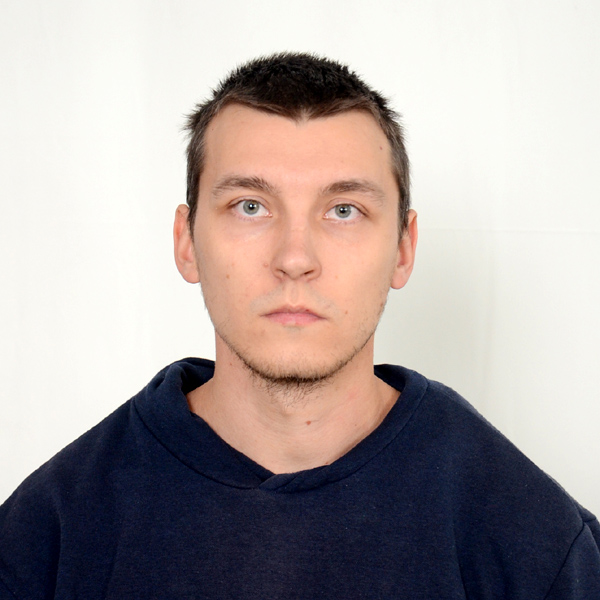
\includegraphics[width=0.8\columnwidth]{photo.jpg}\\[\baselineskip]
\small
\textbf{Mikhail Pedus} \\
pmikhailmail@gmail.com \\
\href{https://github.com/MikhailPedus}{github.com/MikhailPedus}
%(+7) 918 769 37 59 \\
\Sep
\textbf{Address} \\
Kalinigrad \\
Russia \\
\vfill
\end{flushright}
}

%----------------------------------------------------------------------------------------

\begin{document}

\userinformation
\framebreak

%----------------------------------------------------------------------------------------
%	HEADING
%----------------------------------------------------------------------------------------

\cvheading{Mikhail Pedus}
\cvsubheading{Deep Learning Software Engineer}

%----------------------------------------------------------------------------------------
%	ABOUT ME
%----------------------------------------------------------------------------------------

\aboutme{About Me}{
\begin{itemize}
\item Have 10 years of experience in IT industry, software development in computer vision/neural networks algorithms field
\item Able to:
	\begin{itemize}
		\item communicate with international and world-distributed project team. 
		\item work independently and part of team.
		\item communicate in English (intermediate) and Russian (native) 
	\end{itemize}
\end{itemize}
}

%----------------------------------------------------------------------------------------
%	EDUCATION
%----------------------------------------------------------------------------------------

\CVSection{Education}

\CVItem{2010 - 2016, NORTH-CAUCASUS FEDERAL UNIVERSITY
}{master of Computer Science}

\Sep

%----------------------------------------------------------------------------------------
%	EXPERIENCE
%----------------------------------------------------------------------------------------

\CVSection{Experience}

\CVItem{Nov 2019 - present, \textit{AI Framework Developer}, \href{https://intel.com/}{Intel}}
{
Responsibilities:
\begin{itemize}
	\item Development of the \href{https://github.com/openvinotoolkit/vpux-plugin}{VPUX plugin} for \href{https://github.com/openvinotoolkit/openvino}{OpenVino framework}:
	\begin{itemize}
		\item Neural network compiler (using LLVM/MLIR):
		\begin{itemize}
			\item Adding new functionality (new layers/hardware features support)
			\item pre-silicon validation of modern VPU's
		\end{itemize}
		\item Runtime:
		\begin{itemize}
			\item Adding new kernels/layers support on runtime side
		\end{itemize}
	\end{itemize}	
\end{itemize}
Detailed achievements:
\begin{itemize}
	\item Learned how:
	\begin{itemize} 
		\item Vision Processing Unit works on hardware level
		\item neural networks works on low-level
		\item neural networks compilers works
		\item VPU runtime works
	\end{itemize}
	\item Partisipated in the creation/development of the framework for pre-silicon validation:
	\begin{itemize}
		\item Responsible for ensuring that all hardware features of VPU, which supported by hardware, are tested on pre-silicon stage
	\end{itemize}
\end{itemize}
}

\CVItem {Oct 2018 - Oct 2019, \textit{Software developer}, \href{https://en.kalashnikovgroup.ru/}{Kalashnikov Concern}}
{
Responsibilities:
\begin{itemize}
	\item Computer vision algorithms development.
\end{itemize}
Detailed achievements:
\begin{itemize}
	\item Developed a biometric identification algorithm for \href{https://en.kalashnikovgroup.ru/media/perspektivnye-razrabotki/kontsern-kalashnikov-predstavil-sobstvennyy-biometricheskiy-skaner}{biometrical scanner}. Based on palms veins pattern matching
\end{itemize}
}

\CVItem {Nov 2017 - Oct 2018, \textit{Software developer}, \href{https://en.videomatrix.ru/}{Videomatrix}
}
{
Responsibilities:
\begin{itemize}
	\item Computer vision algorithms development.
\end{itemize}
Detailed achievements:
\begin{itemize}
	\item Developed an application/algorithms for \href{https://en.videomatrix.ru/vmx-sila/}{video analitics}. The system recognizes an objects in frame, monitors the appearance and behavior.
\end{itemize}
}

\CVItem {Aug 2012 - Jul 2016, \textit{Software developer}, MMC-Electronics}
{Responsibilities:
\begin{itemize}
	\item People counting algorithms development.
\end{itemize}
Detailed achievements:
\begin{itemize}
	\item Developed and was supporting an algorithm for \href{https://www.youtube.com/watch?v=acb3HhLy3sA}{bus onboard passenger counting system}
\end{itemize}
}

\Sep % Extra whitespace after the end of a major section

\clearpage % Start a new page

\userinformation
\framebreak

%----------------------------------------------------------------------------------------
%	Important SKILLS
%----------------------------------------------------------------------------------------

\CVSection{Soft Skills}
\begin{itemize}
	\item Have good analytical/problem-solving skills, self-initiative and fast to learn new skills/technologies, resourceful, committed, and smart-worker
\end{itemize}
\Sep

%----------------------------------------------------------------------------------------
%	SKILLS
%----------------------------------------------------------------------------------------

\CVSection{Software Development Skills}

%------------------------------------------------

\CVItem{Programming}
{\begin{tabular}{p{0.2\textwidth} p{0.2\textwidth} p{0.2\textwidth}}
\bluebullet C++ &  \bluebullet Linux & \bluebullet Git\\ 
\bluebullet SQL & \bluebullet CMake &  \bluebullet Python\\
\bluebullet DeepLearning & \bluebullet Compilers & \bluebullet OpenVino\\
 \bluebullet OpenCV & \bluebullet LLVM\\
\end{tabular}}

\Sep 

%----------------------------------------------------------------------------------------
%	AWARDS
%----------------------------------------------------------------------------------------

%\CVSection{Achievements}

%------------------------------------------------

%\CVItem{2019, \textit{Idex-2019}, Exhibition}{something about veins pattern recognition}

%------------------------------------------------

%\Sep % Extra whitespace after the end of a major section

%----------------------------------------------------------------------------------------
%	INTERESTS
%----------------------------------------------------------------------------------------

\CVSection{Interests}

%------------------------------------------------

\CVItem{Professional}{neural networks, computer vision, virtual/augmented reality, self-driving car}

%------------------------------------------------

\CVItem{Personal}{Gym, cooking, playing the guitar, hiking}

%------------------------------------------------

\Sep

%----------------------------------------------------------------------------------------

\end{document}
